\item \points{2d}
\textbf{Classical (Unsupervised) EM Implementation.}
For this sub-question, we are only going to consider the $\nexp$ unlabeled examples. Follow the instructions in |src-semi_supervised_em/submission.py| to implement the traditional EM algorithm, and run it on the unlabeled data-set until convergence.
More specifically, please complete the |main| and |run_em| functions. Note: feel free to create your own helper functions in the development of your solution.

Autograder test case |2d-1-basic| can be used to verify a correct implementation. Before running the test case, change line 92 to |skip = False| (this test is skipped by default to make the autograder faster).  It will run three trials and use the provided plotting function to construct a scatter plot of the resulting assignments to clusters (one plot for each trial). The output plot will indicate cluster assignments by assigning unique colors for each cluster (\emph{i.e.,} the cluster which had the highest probability in the final E-step).  Do not submit these plots; they are not graded.\\

Your plots should look similar to the following:

  \begin{figure}[H]
    \centering
    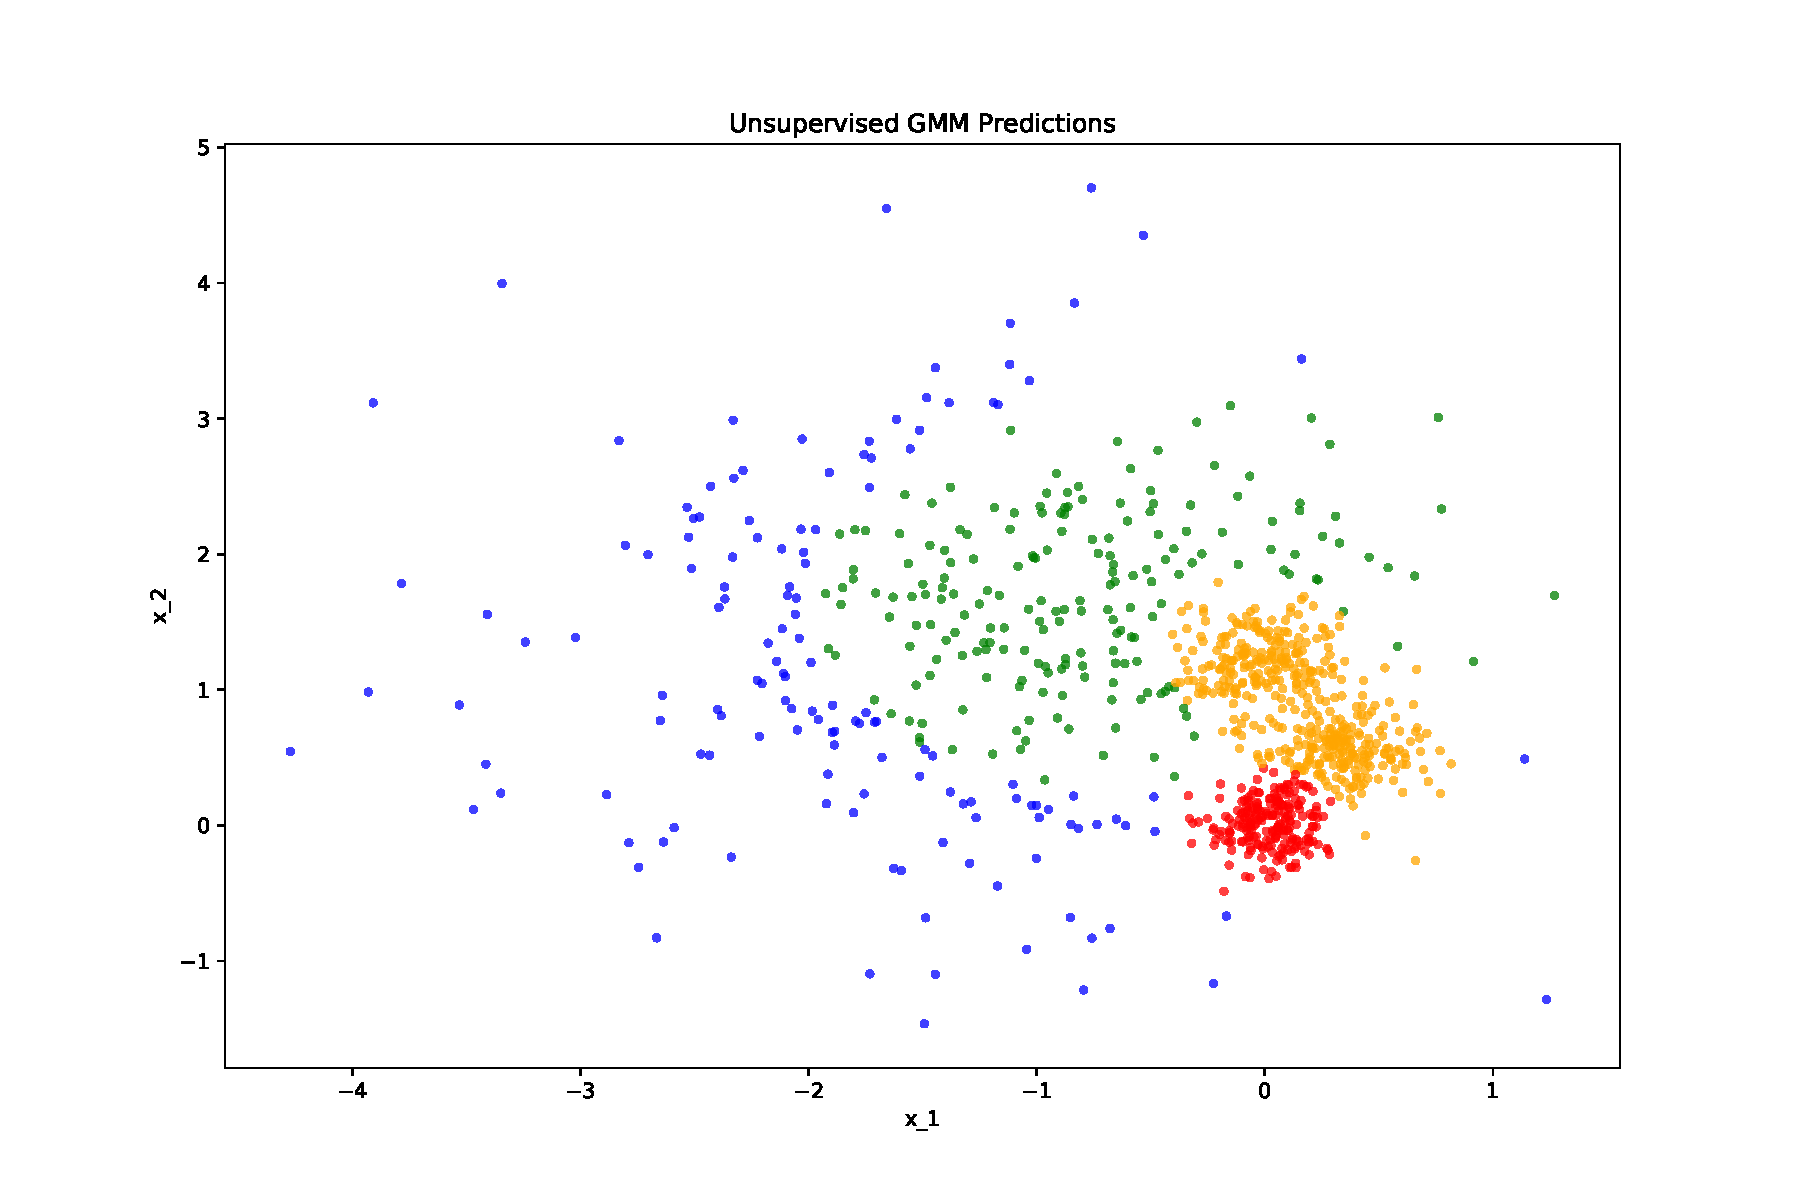
\includegraphics[width=0.3\textwidth]{02-semi_supervised_em/pred_0.pdf}
    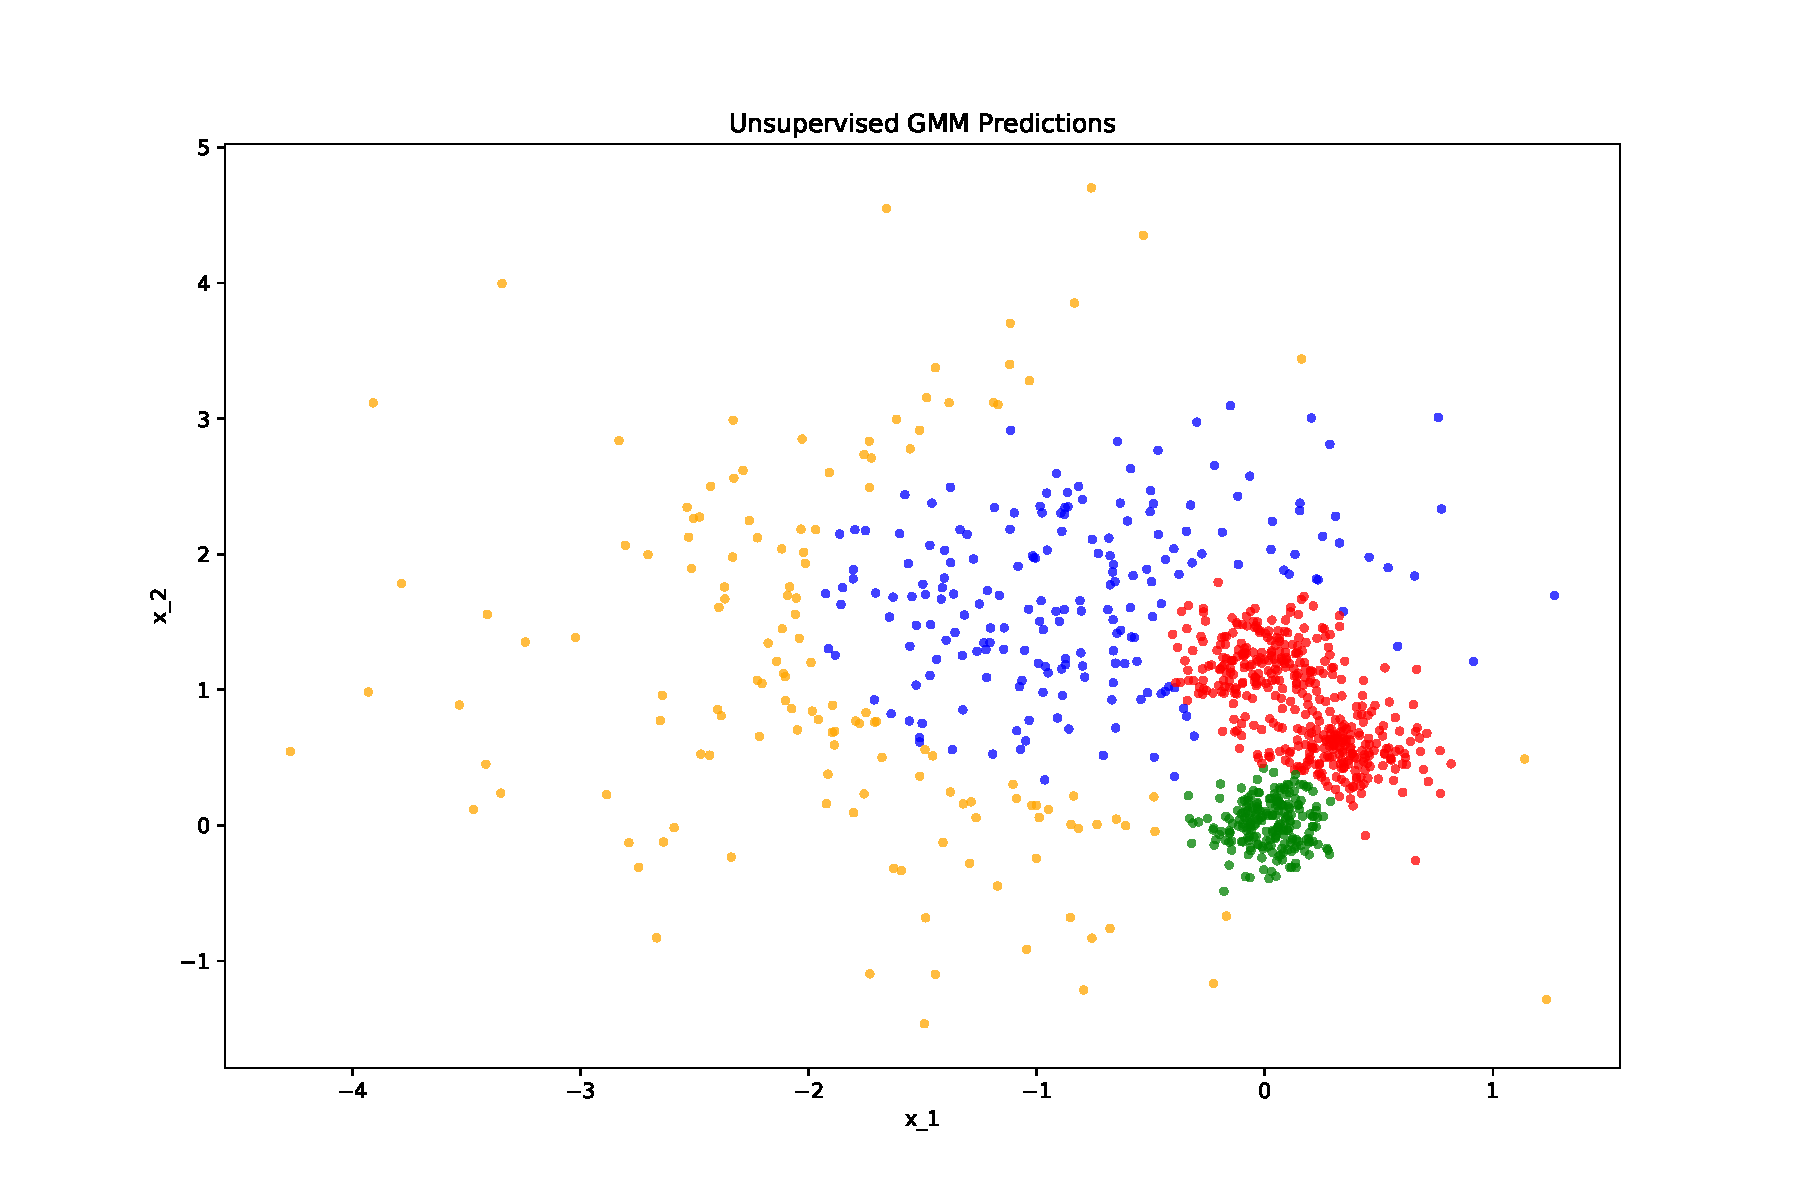
\includegraphics[width=0.3\textwidth]{02-semi_supervised_em/pred_1.pdf}
    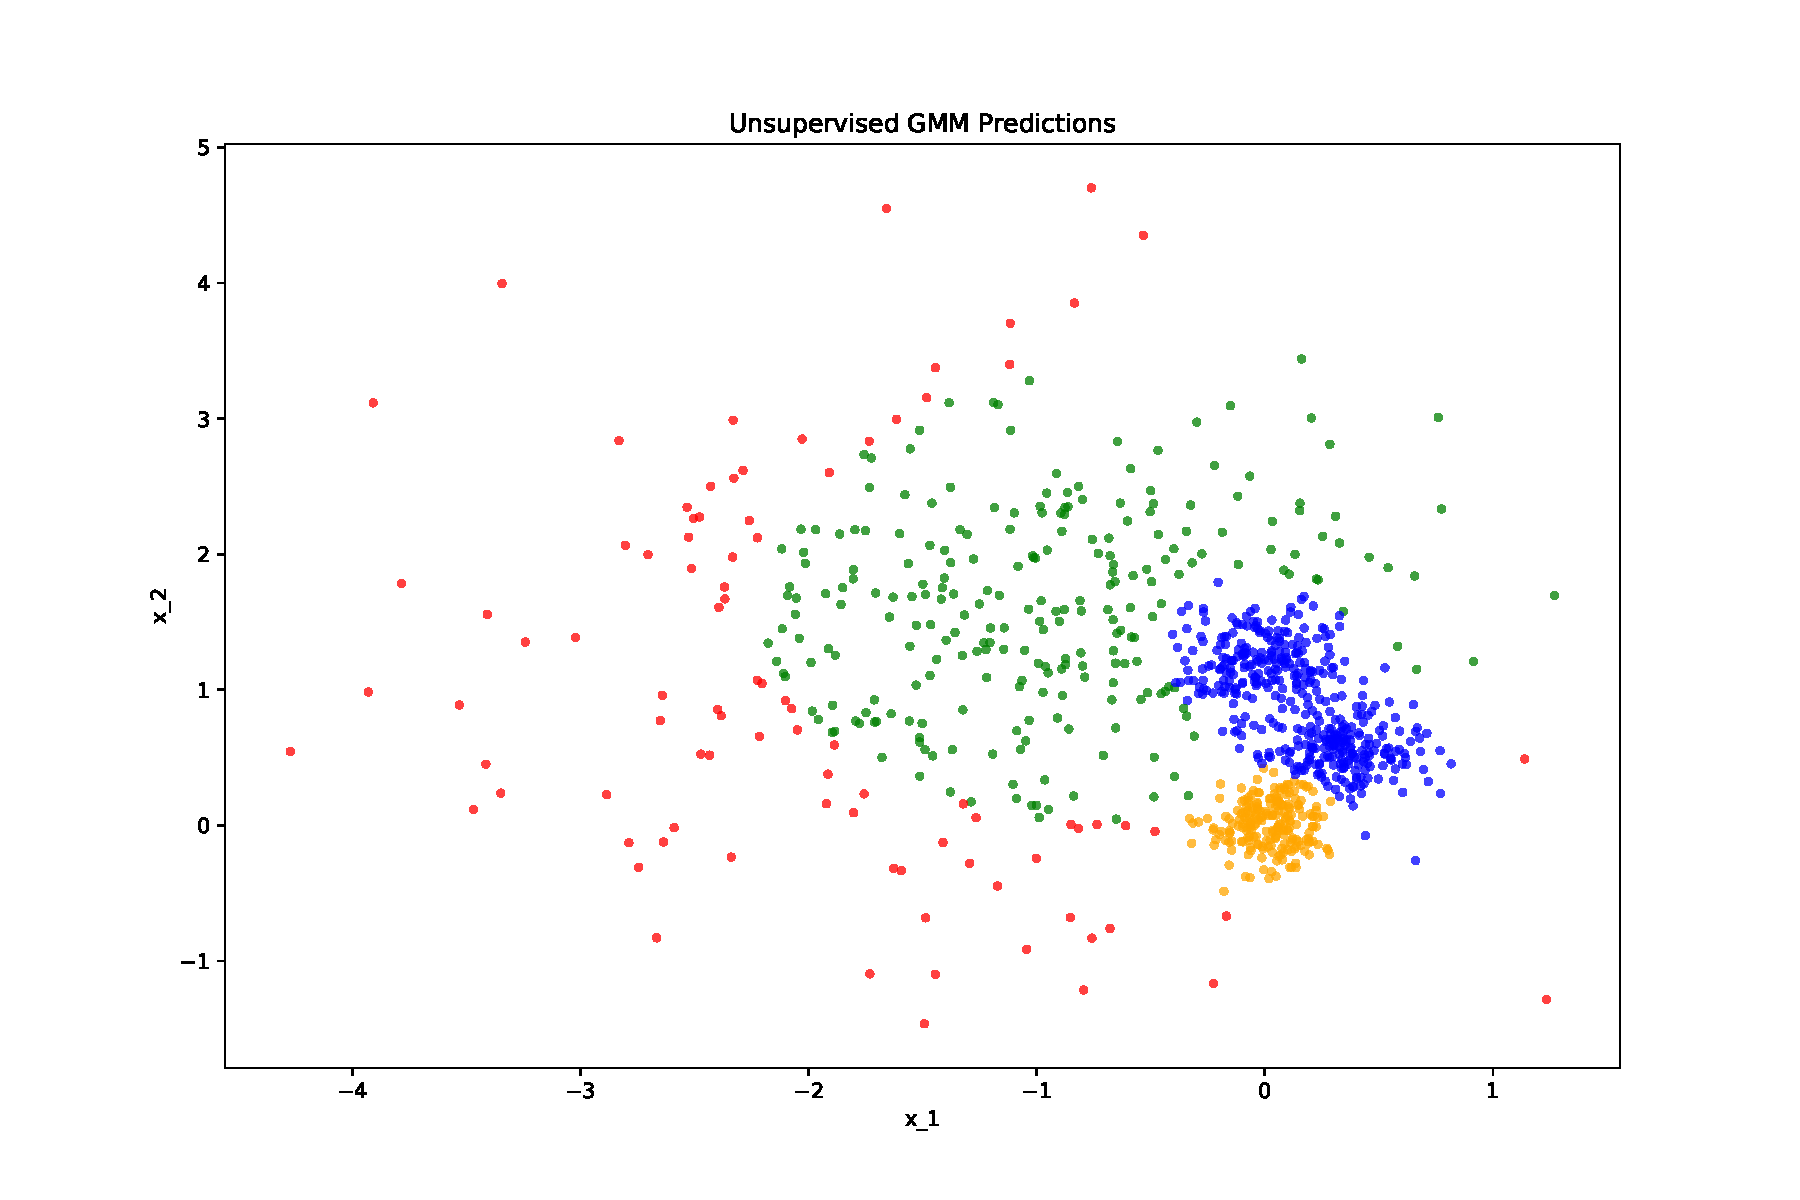
\includegraphics[width=0.3\textwidth]{02-semi_supervised_em/pred_2.pdf}
    \caption{Predictions made by GMM model with unsupervised EM.}
  \end{figure}
